\iffalse
\documentclass[12pt]{article}
\usepackage{graphicx}
%\documentclass[journal,12pt,twocolumn]{IEEEtran}
\usepackage[none]{hyphenat}
\usepackage{graphicx}
\usepackage{listings}
\usepackage[english]{babel}
\usepackage{graphicx}
\usepackage{caption}
\usepackage[parfill]{parskip}
\usepackage{hyperref}
\usepackage{booktabs}
%\usepackage{setspace}\doublespacing\pagestyle{plain}
\def\inputGnumericTable{}
\usepackage{color}                                            %%
    \usepackage{array}                                            %%
    \usepackage{longtable}                                        %%
    \usepackage{calc}                                             %%
    \usepackage{multirow}                                         %%
    \usepackage{hhline}                                           %%
    \usepackage{ifthen}
\usepackage{array}
\usepackage{amsmath}   % for having text in math mode
\usepackage{parallel,enumitem}
\usepackage{listings}
\lstset{
language=tex,
frame=single, 
breaklines=true
}
  
%Following 2 lines were added to remove the blank page at the beginning
\usepackage{atbegshi}% http://ctan.org/pkg/atbegshi
\AtBeginDocument{\AtBeginShipoutNext{\AtBeginShipoutDiscard}}
%
%New macro definitions
\newcommand{\mydet}[1]{\ensuremath{\begin{vmatrix}#1\end{vmatrix}}}
\providecommand{\brak}[1]{\ensuremath{\left(#1\right)}}
\providecommand{\norm}[1]{\left\lVert#1\right\rVert}
\newcommand{\solution}{\noindent \textbf{Solution: }}
\newcommand{\myvec}[1]{\ensuremath{\begin{pmatrix}#1\end{pmatrix}}}
\let\vec\mathbf
\begin{document}
\begin{center}
\title{\textbf{Straight Lines}}
\date{\vspace{-5ex}} %Not to print date automatically
\maketitle
\end{center}
\setcounter{page}{1}
\section*{11$^{th}$ Maths - Chapter 10}
This is Problem-3 from Exercise 10.2
\begin{enumerate}
		\fi
		Line passing through point $\vec{A}=\myvec{0\\0}$ is given by,
\begin{align}
	\vec{n}^\top \brak{\vec{x}-\vec{A}} &= 0\label{eq:11/10/2/31}
\end{align}
Where,
		\begin{align}
			\vec{n} =\myvec{m \\ -1}
		\end{align}
		Substituting $\vec{A}$ and $\vec{n}$ in equation \eqref{eq:11/10/2/31}
		\begin{align}
			\myvec{m & -1}\brak{\vec{x}-\myvec{0\\0}} &=0\\
\implies			\myvec{m & -1}\vec{x} &= 0
		\end{align}
Line segment passing through $\myvec{0\\0}$ with slope $m = 2$ is shown in Fig. \ref{fig:11/10/2/3Fig1}
\begin{figure}[!h]
\begin{center}
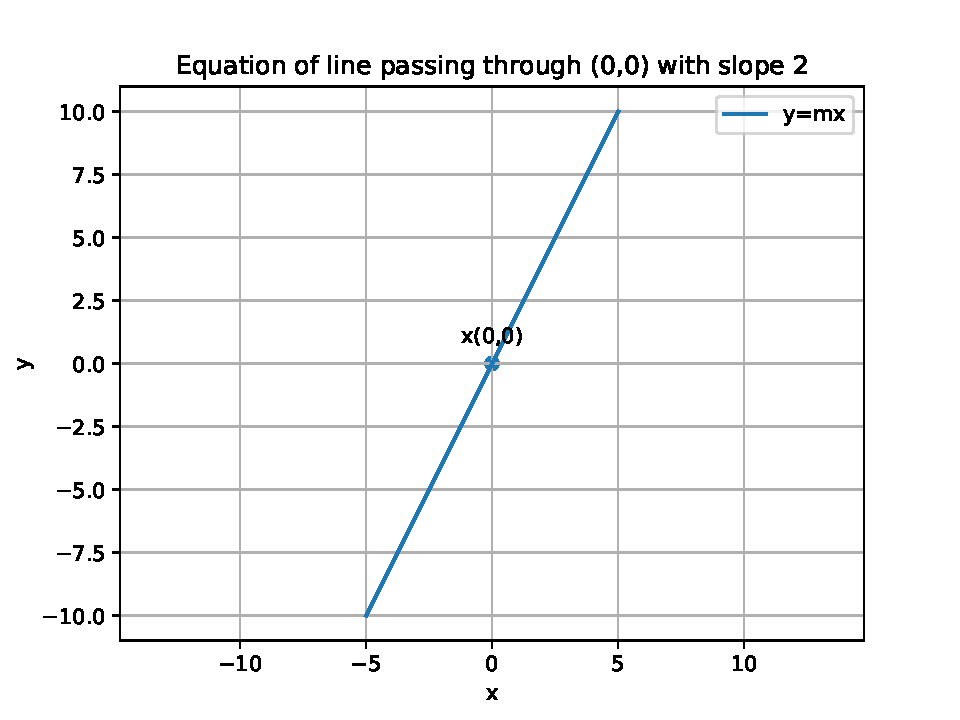
\includegraphics[width=\columnwidth]{chapters/11/10/2/3/figs/fig.pdf}
\end{center}
\caption{}
\label{fig:11/10/2/3Fig1}
\end{figure}
